

\tikzset{every picture/.style={line width=0.75pt}} %set default line width to 0.75pt        

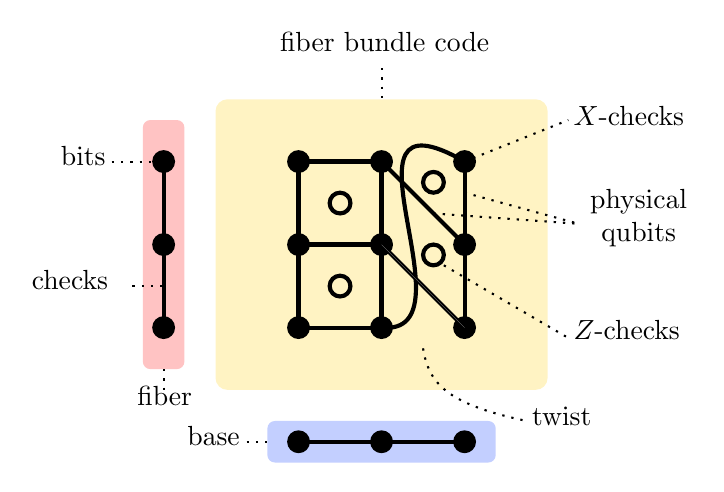
\begin{tikzpicture}[x=0.75pt,y=0.75pt,yscale=-1,xscale=1]
%uncomment if require: \path (0,275); %set diagram left start at 0, and has height of 275

%Rounded Rect [id:dp2507570683512417] 
\draw  [draw opacity=0][fill={rgb, 255:red, 194; green, 206; blue, 255 }  ,fill opacity=0.99 ] (185,228.6) .. controls (185,226.61) and (186.61,225) .. (188.6,225) -- (291.4,225) .. controls (293.39,225) and (295,226.61) .. (295,228.6) -- (295,241.4) .. controls (295,243.39) and (293.39,245) .. (291.4,245) -- (188.6,245) .. controls (186.61,245) and (185,243.39) .. (185,241.4) -- cycle ;
%Rounded Rect [id:dp4432738694856251] 
\draw  [draw opacity=0][fill={rgb, 255:red, 255; green, 194; blue, 194 }  ,fill opacity=0.99 ] (125,83.6) .. controls (125,81.61) and (126.61,80) .. (128.6,80) -- (141.4,80) .. controls (143.39,80) and (145,81.61) .. (145,83.6) -- (145,196.4) .. controls (145,198.39) and (143.39,200) .. (141.4,200) -- (128.6,200) .. controls (126.61,200) and (125,198.39) .. (125,196.4) -- cycle ;
%Rounded Rect [id:dp7720071025717157] 
\draw  [draw opacity=0][fill={rgb, 255:red, 255; green, 243; blue, 194 }  ,fill opacity=0.99 ] (160,75.75) .. controls (160,72.58) and (162.58,70) .. (165.75,70) -- (314.25,70) .. controls (317.42,70) and (320,72.58) .. (320,75.75) -- (320,204.25) .. controls (320,207.42) and (317.42,210) .. (314.25,210) -- (165.75,210) .. controls (162.58,210) and (160,207.42) .. (160,204.25) -- cycle ;
%Straight Lines [id:da5860777651441025] 
\draw [line width=1.5]    (200,100) -- (200,180) ;
%Straight Lines [id:da9228137752045358] 
\draw [line width=1.5]    (240,100) -- (240,180) ;
%Straight Lines [id:da43729330123277244] 
\draw [line width=1.5]    (280,100) -- (280,185) ;
%Shape: Circle [id:dp6618025282379041] 
\draw  [fill={rgb, 255:red, 0; green, 0; blue, 0 }  ,fill opacity=1 ] (195,100) .. controls (195,97.24) and (197.24,95) .. (200,95) .. controls (202.76,95) and (205,97.24) .. (205,100) .. controls (205,102.76) and (202.76,105) .. (200,105) .. controls (197.24,105) and (195,102.76) .. (195,100) -- cycle ;
%Shape: Circle [id:dp8950888733857303] 
\draw  [fill={rgb, 255:red, 0; green, 0; blue, 0 }  ,fill opacity=1 ] (235,100) .. controls (235,97.24) and (237.24,95) .. (240,95) .. controls (242.76,95) and (245,97.24) .. (245,100) .. controls (245,102.76) and (242.76,105) .. (240,105) .. controls (237.24,105) and (235,102.76) .. (235,100) -- cycle ;
%Shape: Circle [id:dp9705906753514444] 
\draw  [fill={rgb, 255:red, 0; green, 0; blue, 0 }  ,fill opacity=1 ] (275,100) .. controls (275,97.24) and (277.24,95) .. (280,95) .. controls (282.76,95) and (285,97.24) .. (285,100) .. controls (285,102.76) and (282.76,105) .. (280,105) .. controls (277.24,105) and (275,102.76) .. (275,100) -- cycle ;
%Shape: Circle [id:dp5577996464413779] 
\draw  [fill={rgb, 255:red, 0; green, 0; blue, 0 }  ,fill opacity=1 ] (195,140) .. controls (195,137.24) and (197.24,135) .. (200,135) .. controls (202.76,135) and (205,137.24) .. (205,140) .. controls (205,142.76) and (202.76,145) .. (200,145) .. controls (197.24,145) and (195,142.76) .. (195,140) -- cycle ;
%Shape: Circle [id:dp2255574832912377] 
\draw  [fill={rgb, 255:red, 0; green, 0; blue, 0 }  ,fill opacity=1 ] (235,140) .. controls (235,137.24) and (237.24,135) .. (240,135) .. controls (242.76,135) and (245,137.24) .. (245,140) .. controls (245,142.76) and (242.76,145) .. (240,145) .. controls (237.24,145) and (235,142.76) .. (235,140) -- cycle ;
%Shape: Circle [id:dp24559158536904913] 
\draw  [fill={rgb, 255:red, 0; green, 0; blue, 0 }  ,fill opacity=1 ] (275,140) .. controls (275,137.24) and (277.24,135) .. (280,135) .. controls (282.76,135) and (285,137.24) .. (285,140) .. controls (285,142.76) and (282.76,145) .. (280,145) .. controls (277.24,145) and (275,142.76) .. (275,140) -- cycle ;
%Shape: Circle [id:dp4755982750247709] 
\draw  [fill={rgb, 255:red, 0; green, 0; blue, 0 }  ,fill opacity=1 ] (195,180) .. controls (195,177.24) and (197.24,175) .. (200,175) .. controls (202.76,175) and (205,177.24) .. (205,180) .. controls (205,182.76) and (202.76,185) .. (200,185) .. controls (197.24,185) and (195,182.76) .. (195,180) -- cycle ;
%Shape: Circle [id:dp5490092987095487] 
\draw  [fill={rgb, 255:red, 0; green, 0; blue, 0 }  ,fill opacity=1 ] (235,180) .. controls (235,177.24) and (237.24,175) .. (240,175) .. controls (242.76,175) and (245,177.24) .. (245,180) .. controls (245,182.76) and (242.76,185) .. (240,185) .. controls (237.24,185) and (235,182.76) .. (235,180) -- cycle ;
%Shape: Circle [id:dp9613260046209995] 
\draw  [fill={rgb, 255:red, 0; green, 0; blue, 0 }  ,fill opacity=1 ] (275,180) .. controls (275,177.24) and (277.24,175) .. (280,175) .. controls (282.76,175) and (285,177.24) .. (285,180) .. controls (285,182.76) and (282.76,185) .. (280,185) .. controls (277.24,185) and (275,182.76) .. (275,180) -- cycle ;

%Shape: Circle [id:dp75449725785472] 
\draw  [line width=1.5]  (215,120) .. controls (215,117.24) and (217.24,115) .. (220,115) .. controls (222.76,115) and (225,117.24) .. (225,120) .. controls (225,122.76) and (222.76,125) .. (220,125) .. controls (217.24,125) and (215,122.76) .. (215,120) -- cycle ;
%Shape: Circle [id:dp1194269851204306] 
\draw  [line width=1.5]  (260,145) .. controls (260,142.24) and (262.24,140) .. (265,140) .. controls (267.76,140) and (270,142.24) .. (270,145) .. controls (270,147.76) and (267.76,150) .. (265,150) .. controls (262.24,150) and (260,147.76) .. (260,145) -- cycle ;
%Shape: Circle [id:dp35190266633136913] 
\draw  [line width=1.5]  (215,160) .. controls (215,157.24) and (217.24,155) .. (220,155) .. controls (222.76,155) and (225,157.24) .. (225,160) .. controls (225,162.76) and (222.76,165) .. (220,165) .. controls (217.24,165) and (215,162.76) .. (215,160) -- cycle ;
%Shape: Circle [id:dp32839477834388586] 
\draw  [line width=1.5]  (260,110) .. controls (260,107.24) and (262.24,105) .. (265,105) .. controls (267.76,105) and (270,107.24) .. (270,110) .. controls (270,112.76) and (267.76,115) .. (265,115) .. controls (262.24,115) and (260,112.76) .. (260,110) -- cycle ;
%Straight Lines [id:da057598114350428053] 
\draw [line width=1.5]    (135,100) -- (135,180) ;
%Shape: Circle [id:dp8842377331787077] 
\draw  [fill={rgb, 255:red, 0; green, 0; blue, 0 }  ,fill opacity=1 ] (130,100) .. controls (130,97.24) and (132.24,95) .. (135,95) .. controls (137.76,95) and (140,97.24) .. (140,100) .. controls (140,102.76) and (137.76,105) .. (135,105) .. controls (132.24,105) and (130,102.76) .. (130,100) -- cycle ;
%Shape: Circle [id:dp14889082824519062] 
\draw  [fill={rgb, 255:red, 0; green, 0; blue, 0 }  ,fill opacity=1 ] (130,140) .. controls (130,137.24) and (132.24,135) .. (135,135) .. controls (137.76,135) and (140,137.24) .. (140,140) .. controls (140,142.76) and (137.76,145) .. (135,145) .. controls (132.24,145) and (130,142.76) .. (130,140) -- cycle ;
%Shape: Circle [id:dp09323821385400355] 
\draw  [fill={rgb, 255:red, 0; green, 0; blue, 0 }  ,fill opacity=1 ] (130,180) .. controls (130,177.24) and (132.24,175) .. (135,175) .. controls (137.76,175) and (140,177.24) .. (140,180) .. controls (140,182.76) and (137.76,185) .. (135,185) .. controls (132.24,185) and (130,182.76) .. (130,180) -- cycle ;
%Straight Lines [id:da22259915305695266] 
\draw [line width=1.5]    (200,235) -- (285,235) ;
%Shape: Circle [id:dp5065267898782895] 
\draw  [fill={rgb, 255:red, 0; green, 0; blue, 0 }  ,fill opacity=1 ] (195,235) .. controls (195,232.24) and (197.24,230) .. (200,230) .. controls (202.76,230) and (205,232.24) .. (205,235) .. controls (205,237.76) and (202.76,240) .. (200,240) .. controls (197.24,240) and (195,237.76) .. (195,235) -- cycle ;
%Shape: Circle [id:dp8042127437497666] 
\draw  [fill={rgb, 255:red, 0; green, 0; blue, 0 }  ,fill opacity=1 ] (235,235) .. controls (235,232.24) and (237.24,230) .. (240,230) .. controls (242.76,230) and (245,232.24) .. (245,235) .. controls (245,237.76) and (242.76,240) .. (240,240) .. controls (237.24,240) and (235,237.76) .. (235,235) -- cycle ;
%Straight Lines [id:da7882166530542396] 
\draw  [dash pattern={on 0.84pt off 2.51pt}]  (110,100) -- (130,100) ;
%Straight Lines [id:da6912991650470606] 
\draw  [dash pattern={on 0.84pt off 2.51pt}]  (120,160) -- (135,160) ;
%Straight Lines [id:da9843251757025941] 
\draw  [dash pattern={on 0.84pt off 2.51pt}]  (280,100) -- (330,80) ;
%Straight Lines [id:da03275132500810485] 
\draw  [dash pattern={on 0.84pt off 2.51pt}]  (270,150) -- (330,185) ;
%Straight Lines [id:da34887226429612284] 
\draw  [dash pattern={on 0.84pt off 2.51pt}]  (265,125) -- (335,130) ;
%Straight Lines [id:da17899042228177908] 
\draw  [dash pattern={on 0.84pt off 2.51pt}]  (280,115) -- (335,130) ;
%Straight Lines [id:da39960611742809093] 
\draw  [dash pattern={on 0.84pt off 2.51pt}]  (135,200) -- (135,210) ;
%Straight Lines [id:da5541317194100692] 
\draw  [dash pattern={on 0.84pt off 2.51pt}]  (175,235) -- (185,235) ;
%Straight Lines [id:da41532796703836006] 
\draw  [dash pattern={on 0.84pt off 2.51pt}]  (240,55) -- (240,70) ;
%Shape: Circle [id:dp49727494677863415] 
\draw  [fill={rgb, 255:red, 0; green, 0; blue, 0 }  ,fill opacity=1 ] (275,235) .. controls (275,232.24) and (277.24,230) .. (280,230) .. controls (282.76,230) and (285,232.24) .. (285,235) .. controls (285,237.76) and (282.76,240) .. (280,240) .. controls (277.24,240) and (275,237.76) .. (275,235) -- cycle ;
%Straight Lines [id:da8793737196729381] 
\draw [line width=1.5]    (240,140) -- (280,180) ;
%Straight Lines [id:da816437026632451] 
\draw [line width=1.5]    (240,100) -- (280,140) ;
%Curve Lines [id:da8936846802404004] 
\draw [line width=1.5]    (280,100) .. controls (211.8,60.7) and (287,184.3) .. (240,180) ;
%Straight Lines [id:da08435083022367085] 
\draw [line width=1.5]    (200,180) -- (240,180) ;
%Straight Lines [id:da32136686692442384] 
\draw [line width=1.5]    (200,140) -- (240,140) ;
%Straight Lines [id:da5026425248072095] 
\draw [line width=1.5]    (200,100) -- (240,100) ;
%Straight Lines [id:da28915883628585526] 
\draw [draw opacity=0][fill={rgb, 255:red, 255; green, 255; blue, 255 }  ,fill opacity=1 ][line width=2.25]    (240,140) -- (280,180) ;
%Curve Lines [id:da5044383487479938] 
\draw  [dash pattern={on 0.84pt off 2.51pt}]  (260,190) .. controls (262.6,206.1) and (270.2,216.7) .. (310,225) ;

% Text Node
\draw (186,36) node [anchor=north west][inner sep=0.75pt]   [align=left] {\begin{minipage}[lt]{80.98392pt}\setlength\topsep{0pt}
\begin{center}
fiber bundle code
\end{center}

\end{minipage}};
% Text Node
\draw (141,226) node [anchor=north west][inner sep=0.75pt]   [align=left] {\begin{minipage}[lt]{24.841216pt}\setlength\topsep{0pt}
\begin{center}
base
\end{center}

\end{minipage}};
% Text Node
\draw (84,91) node [anchor=north west][inner sep=0.75pt]   [align=left] {bits};
% Text Node
\draw (70,151) node [anchor=north west][inner sep=0.75pt]   [align=left] {checks};
% Text Node
\draw (331,72) node [anchor=north west][inner sep=0.75pt]   [align=left] {$\displaystyle X$-checks};
% Text Node
\draw (331,175) node [anchor=north west][inner sep=0.75pt]   [align=left] {$\displaystyle Z$-checks};
% Text Node
\draw (336,112) node [anchor=north west][inner sep=0.75pt]   [align=left] {\begin{minipage}[lt]{39.578108pt}\setlength\topsep{0pt}
\begin{center}
physical\\qubits
\end{center}

\end{minipage}};
% Text Node
\draw (119,207) node [anchor=north west][inner sep=0.75pt]   [align=left] {\begin{minipage}[lt]{22.567500000000003pt}\setlength\topsep{0pt}
\begin{center}
fiber
\end{center}

\end{minipage}};
% Text Node
\draw (311,217) node [anchor=north west][inner sep=0.75pt]   [align=left] {twist};


\end{tikzpicture}
